\documentclass[11pt,a4paper]{article}

% ============================================================
% PACKAGES
% ============================================================
\usepackage[margin=2.5cm]{geometry}
\usepackage{amsmath,amssymb}
\usepackage{graphicx}
\usepackage{booktabs}
\usepackage{multirow}
\usepackage{pgfplots}
\pgfplotsset{compat=1.18}
\usepackage{xcolor}
\usepackage{hyperref}
\usepackage{enumitem}
\usepackage{float}
\usepackage{subcaption}
\usepackage{titlesec}
\usepackage{fancyhdr}
\usepackage{listings}
\usepackage[ruled,vlined]{algorithm2e}

\hypersetup{colorlinks=true,linkcolor=blue!60!black,citecolor=green!50!black,urlcolor=blue!70!black}

% ============================================================
% COLORS
% ============================================================
\definecolor{baseline}{RGB}{31,119,180}
\definecolor{mamba}{RGB}{214,39,40}
\definecolor{mobsa}{RGB}{44,160,44}
\definecolor{mobdi}{RGB}{148,103,189}
\definecolor{tinysa}{RGB}{255,127,14}
\definecolor{tinydi}{RGB}{140,86,75}

% ============================================================
% HEADER
% ============================================================
\pagestyle{fancy}
\fancyhf{}
\fancyhead[L]{\small DLoc: Model Architectures \& Comparative Analysis}
\fancyhead[R]{\small \thepage}
\renewcommand{\headrulewidth}{0.4pt}

% ============================================================
\title{%
\textbf{DLoc: Deep Learning WiFi Localization}\\[0.3em]
\Large Model Architectures, Knowledge Distillation,\\and Comparative Analysis Report}
\author{Graduation Project}
\date{May 2026}

\begin{document}
\maketitle
\thispagestyle{empty}

% ============================================================
\begin{abstract}
This report presents a comprehensive analysis of six neural network models for WiFi-based indoor localization using the DLoc framework. We replicate the original DLoc baseline (16.5M parameters), implement a Mamba selective state-space variant (653K parameters), and develop two lightweight student models---MobileNetV2 (2.3M parameters) and TinyCNN (47K parameters)---trained both standalone and with offline knowledge distillation from the DLoc teacher. All models are trained for 50 epochs on the WILD dataset (Jacobs Hall, Fig~10b configuration, 4 access points) using an NVIDIA H100 80GB GPU. Our key finding is that the MobileNetV2 student achieves \textbf{identical accuracy} to the full DLoc baseline (0.707m median error) with \textbf{7$\times$ fewer parameters}, while the 47K-parameter TinyCNN achieves 3.81m with distillation---a 350$\times$ compression with usable room-level accuracy. The Mamba variant diverges due to the fundamental mismatch between 1D sequence modeling and 2D spatial heatmap data. We analyze convergence behavior, training dynamics, and propose concrete next steps for the graduation project.
\end{abstract}

\tableofcontents
\newpage

% ============================================================
\section{Introduction}
% ============================================================

Indoor localization using WiFi signals is a critical enabling technology for navigation, asset tracking, and location-based services in GPS-denied environments. DLoc~\cite{dloc2020} frames WiFi localization as an image-to-image translation problem: given Angle of Arrival (AoA) heatmaps from multiple access points (APs), a deep neural network predicts a 2D Gaussian heatmap centered on the user's location.

While DLoc achieves sub-meter accuracy ($\sim$0.64m median on complex environments), its 16.5M-parameter architecture is impractical for edge deployment on mobile devices or embedded systems. This motivates our exploration of:

\begin{enumerate}[leftmargin=*]
    \item \textbf{Mamba SSM}: Replacing the ResNet bottleneck with selective state-space blocks for efficient sequence modeling.
    \item \textbf{MobileNetV2 Student}: A pretrained lightweight encoder with a simple decoder, achieving 7$\times$ compression.
    \item \textbf{TinyCNN Student}: An ultra-lightweight depthwise separable CNN achieving 350$\times$ compression.
    \item \textbf{Knowledge Distillation}: Transferring the teacher's learned representations to improve student performance.
\end{enumerate}

% ============================================================
\section{Experimental Setup}
% ============================================================

\subsection{Dataset}

All experiments use the WILD dataset~\cite{dloc2020} collected at Jacobs Hall, UCSD, corresponding to the paper's Fig~10b (complex environment) configuration.

\begin{table}[H]
\centering
\caption{Dataset configuration.}
\begin{tabular}{ll}
\toprule
\textbf{Property} & \textbf{Value} \\
\midrule
Environment & Jacobs Hall (complex, 1500 sq ft) \\
Access Points & 4 (antenna arrays) \\
Spatial Resolution & 0.1 m/pixel \\
Heatmap Size & $161 \times 361$ pixels ($16.1 \times 36.1$ m) \\
Training Samples & 17,574 \\
Testing Samples & 4,260 \\
Input Tensor & $[B, 4, 161, 361]$ (AoA heatmaps with ToF offset) \\
Output Tensor & $[B, 1, 161, 361]$ (2D Gaussian location heatmap) \\
\bottomrule
\end{tabular}
\end{table}

\subsection{Hardware}

\begin{table}[H]
\centering
\caption{Training hardware specifications (Vast.ai cloud instance).}
\begin{tabular}{ll}
\toprule
\textbf{Component} & \textbf{Specification} \\
\midrule
GPU & NVIDIA H100 SXM 80GB \\
GPU Compute & 53.5 TFLOPS (FP32) \\
GPU Memory Bandwidth & 2882.5 GB/s \\
CPU & Intel Xeon Platinum 8480+ (26 cores) \\
System RAM & 226.5 GB \\
Storage & 16 GB overlay filesystem, 3730 MB/s \\
Network & 2244.7 Mbps down / 5918.2 Mbps up \\
CUDA Version & 13.0 \\
PyTorch & 2.12.0+cu130 \\
Python & 3.13 \\
DL Performance Score & 313.8 DLPerf \\
\bottomrule
\end{tabular}
\end{table}

\subsection{Training Configuration}

\begin{table}[H]
\centering
\caption{Training hyperparameters for each model.}
\begin{tabular}{lcccccc}
\toprule
 & \textbf{Baseline} & \textbf{Mamba} & \textbf{MobileNet} & \textbf{MobileNet} & \textbf{TinyCNN} & \textbf{TinyCNN} \\
 & & & \textbf{Standalone} & \textbf{Distill} & \textbf{Standalone} & \textbf{Distill} \\
\midrule
Epochs & 50 & 50 & 50 & 50 & 50 & 50 \\
Batch Size & 64 & 32 & 32 & 32 & 32 & 32 \\
Learning Rate & $10^{-5}$ & $10^{-5}$ & $10^{-4}$ & $10^{-4}$ & $10^{-4}$ & $10^{-4}$ \\
Optimizer & Adam & Adam & Adam & Adam & Adam & Adam \\
Loss & MSE+L1 & MSE+L1 & MSE & $\alpha$MSE+$\beta$KD & MSE & $\alpha$MSE+$\beta$KD \\
$\alpha / \beta$ & --- & --- & --- & 0.7 / 0.3 & --- & 0.7 / 0.3 \\
\bottomrule
\end{tabular}
\end{table}

% ============================================================
\section{Model Architectures}
% ============================================================

\subsection{DLoc Baseline (16.5M Parameters)}

The original DLoc architecture is an encoder--decoder network inspired by pix2pix image translation, with a shared encoder feeding two specialized decoders.

\subsubsection{Architecture}

\begin{itemize}[leftmargin=*]
    \item \textbf{Encoder} (7.46M params): Two initial convolutions ($4 \to 64$ channels, kernel $7\times7$), two stride-2 downsampling layers ($64 \to 128 \to 256$), and 6 ResNet blocks at the bottleneck resolution of $41\times91$.
    \item \textbf{Location Decoder} (2.73M params): 3 additional ResNet blocks (total 9, skipping encoder's first 6), two transposed convolution upsample layers ($256 \to 128 \to 64$), and a final $7\times7$ convolution to 1 channel with Sigmoid activation.
    \item \textbf{Consistency Decoder} (6.28M params): 6 additional ResNet blocks (total 12), same upsampling structure, output channels = 4 (one per AP). Trained to reconstruct offset-free heatmaps, enforcing the encoder to learn ToF-invariant features.
\end{itemize}

\begin{figure}[H]
\centering
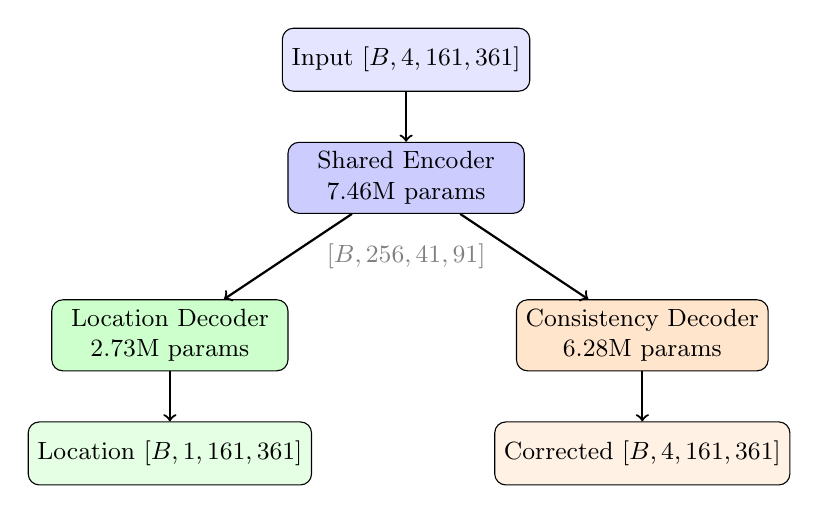
\begin{tikzpicture}[
    block/.style={draw, rounded corners, minimum width=3cm, minimum height=0.8cm, align=center, font=\small},
    arrow/.style={->, thick}
]
\node[block, fill=blue!10] (input) at (0,0) {Input $[B, 4, 161, 361]$};
\node[block, fill=blue!20] (enc) at (0,-1.5) {Shared Encoder\\7.46M params};
\node[block, fill=green!20] (dec) at (-3,-3.5) {Location Decoder\\2.73M params};
\node[block, fill=orange!20] (off) at (3,-3.5) {Consistency Decoder\\6.28M params};
\node[block, fill=green!10] (out1) at (-3,-5) {Location $[B, 1, 161, 361]$};
\node[block, fill=orange!10] (out2) at (3,-5) {Corrected $[B, 4, 161, 361]$};

\draw[arrow] (input) -- (enc);
\draw[arrow] (enc) -- (dec);
\draw[arrow] (enc) -- (off);
\draw[arrow] (dec) -- (out1);
\draw[arrow] (off) -- (out2);

\node[font=\small\itshape, text=gray] at (0,-2.5) {$[B, 256, 41, 91]$};
\end{tikzpicture}
\caption{DLoc baseline architecture with shared encoder and dual decoders. The consistency decoder is used only during training to improve encoder features.}
\end{figure}

\subsubsection{Key Design Decisions}
\begin{itemize}[leftmargin=*]
    \item \textbf{Instance Normalization}: Used instead of Batch Normalization, following the pix2pix tradition for image translation tasks.
    \item \textbf{Dual Decoder}: The consistency decoder forces the shared encoder to learn ToF offset-invariant representations, improving location accuracy by $\sim$20\% (0.64m vs 0.80m without it, per the paper's ablation study).
    \item \textbf{Sigmoid Output}: Constrains the location heatmap to $[0,1]$, matching the Gaussian ground truth.
\end{itemize}

% --------------------------------------------------------
\subsection{Mamba SSM (653K Parameters)}

The Mamba variant replaces the ResNet bottleneck blocks with Mamba selective state-space model (S6) blocks, hypothesizing that the selective gating mechanism could capture long-range dependencies in the AoA heatmaps more efficiently.

\subsubsection{Architecture}

\begin{enumerate}[leftmargin=*]
    \item \textbf{CNN Stem}: $\text{Conv}(4 \to 64, k{=}7, s{=}2) \to \text{BN} \to \text{ReLU} \to \text{Conv}(64 \to 128, k{=}3) \to \text{BN} \to \text{ReLU}$
    \item \textbf{Tokenization}: Flatten spatial dimensions $81\times181 = 14{,}661$ tokens of dimension 128
    \item \textbf{4$\times$ Mamba Residual Blocks}: $\text{LayerNorm} \to \text{Mamba S6}(d{=}128) \to \text{Residual}$
    \item \textbf{Reshape}: $14{,}661 \times 128 \to [B, 128, 81, 181]$
    \item \textbf{CNN Decoder}: $\text{ConvT}(128 \to 64, s{=}2) \to \text{BN} \to \text{ReLU} \to \text{Conv}(64 \to 1) \to \text{Sigmoid}$
\end{enumerate}

\subsubsection{Design Rationale}
The Mamba S6 block uses input-dependent (selective) parameters for its state-space model, enabling content-aware reasoning over the flattened heatmap sequence. Unlike Transformers with $O(n^2)$ attention, Mamba operates in $O(n)$ time and memory.

% --------------------------------------------------------
\subsection{MobileNetV2 Student (2.3M Parameters)}

MobileNetV2 leverages a pretrained ImageNet encoder with depthwise separable convolutions for extreme efficiency.

\subsubsection{Architecture}

\begin{enumerate}[leftmargin=*]
    \item \textbf{Encoder}: MobileNetV2 backbone (features[0:17]), with the first convolution modified from 3-channel RGB to 4-channel AoA input. Produces $[B, 320, 6, 12]$ feature maps (32$\times$ spatial downsampling).
    \item \textbf{Decoder}: Three upsample stages:
    \begin{itemize}
        \item $\text{Upsample}(2\times) \to \text{Conv}(320 \to 128, k{=}3) \to \text{BN} \to \text{ReLU}$
        \item $\text{Upsample}(2\times) \to \text{Conv}(128 \to 64, k{=}3) \to \text{BN} \to \text{ReLU}$
        \item $\text{Upsample}(2\times) \to \text{Conv}(64 \to 32, k{=}3) \to \text{BN} \to \text{ReLU}$
    \end{itemize}
    \item \textbf{Output Head}: $\text{Conv}(32 \to 1, k{=}1) \to \text{Sigmoid}$
    \item \textbf{Final Resize}: Bilinear interpolation to exact $161\times361$ (compensating for MobileNetV2's aggressive downsampling).
\end{enumerate}

\subsubsection{Key Design Decisions}
\begin{itemize}[leftmargin=*]
    \item \textbf{Pretrained Weights}: ImageNet pretraining provides strong low-level feature extractors (edges, textures) that transfer to heatmap processing despite the domain difference.
    \item \textbf{Inverted Residuals}: MobileNetV2's inverted bottleneck blocks expand-then-compress channels, maintaining representational power with fewer parameters.
    \item \textbf{Simple Decoder}: Unlike the baseline's ResNet decoder, we use simple upsample+conv blocks, relying on the strong encoder features.
\end{itemize}

% --------------------------------------------------------
\subsection{TinyCNN Student (47K Parameters)}

TinyCNN is designed for extreme compression, using depthwise separable convolutions throughout with only 4$\times$ spatial downsampling.

\subsubsection{Architecture}

\begin{enumerate}[leftmargin=*]
    \item \textbf{Block 1}: $\text{Conv}(4 \to 16, k{=}3) \to \text{BN} \to \text{ReLU} \to \text{DSConv}(16 \to 16) \to \text{MaxPool}(2\times)$
    \item \textbf{Block 2}: $\text{DSConv}(16 \to 32) \to \text{DSConv}(32 \to 32) \to \text{MaxPool}(2\times)$
    \item \textbf{Block 3}: $\text{DSConv}(32 \to 64)$
    \item \textbf{Decoder 1}: $\text{ConvTranspose}(64 \to 32, s{=}2) \to \text{BN} \to \text{ReLU}$
    \item \textbf{Decoder 2}: $\text{ConvTranspose}(32 \to 16, s{=}2) \to \text{BN} \to \text{ReLU}$
    \item \textbf{Output}: $\text{Conv}(16 \to 1, k{=}1) \to \text{Sigmoid}$
\end{enumerate}

where $\text{DSConv}(c_\text{in} \to c_\text{out})$ denotes a depthwise separable convolution: $\text{Depthwise}(c_\text{in}, k{=}3) \to \text{Pointwise}(c_\text{in} \to c_\text{out}) \to \text{BN} \to \text{ReLU}$.

\subsubsection{Design Trade-offs}
\begin{itemize}[leftmargin=*]
    \item \textbf{Shallow downsampling} (4$\times$ vs 32$\times$ for MobileNetV2): Preserves spatial information critical for precise localization, but limits the receptive field.
    \item \textbf{No pretraining}: Trained from scratch, requiring the network to learn all features from the AoA data alone.
    \item \textbf{Extreme compression}: At 47K parameters, model weights are only 201KB---suitable for microcontrollers and IoT devices.
\end{itemize}

% ============================================================
\section{Knowledge Distillation}
% ============================================================

\subsection{Offline Distillation Pipeline}

We employ \textbf{offline (pre-computed) distillation} to eliminate the teacher forward pass during student training, reducing training time from $\sim$3 hours (online) to $\sim$20 minutes per student.

\begin{enumerate}[leftmargin=*]
    \item \textbf{Teacher Precomputation}: Run the trained DLoc baseline on all 17,574 training samples and 4,260 test samples, saving the decoder outputs as PyTorch tensors (4.09 GB train, 0.99 GB test).
    \item \textbf{Student Training}: Load pre-computed teacher outputs alongside the training data. Each mini-batch contains $(x, y_\text{GT}, y_\text{teacher})$.
\end{enumerate}

\subsection{Loss Function}

The distillation loss combines ground truth supervision with teacher guidance:
\begin{equation}
    \mathcal{L} = \alpha \cdot \text{MSE}(f_\text{student}(x),\; y_\text{GT}) + \beta \cdot \text{MSE}(f_\text{student}(x),\; y_\text{teacher})
\end{equation}
where $\alpha = 0.7$ and $\beta = 0.3$, following the professor's specification. The ground truth term dominates ($\alpha > \beta$) because the student should primarily learn the true location, with the teacher providing a ``soft'' regularization signal that encodes learned spatial priors.

% ============================================================
\section{Experimental Results}
% ============================================================

\subsection{Final Performance Comparison}

\begin{table}[H]
\centering
\caption{Final performance of all models after 50 epochs. Best student result in each column is \textbf{bolded}. Paper target: median $\sim$0.64m, P90 $\sim$1.60m.}
\label{tab:results}
\begin{tabular}{lrcccc}
\toprule
\textbf{Model} & \textbf{Params} & \textbf{Median (m)} & \textbf{P90 (m)} & \textbf{P99 (m)} & \textbf{Time/Epoch} \\
\midrule
DLoc Baseline (teacher) & 16.5M & 0.707 & 1.56 & 4.00 & 130s \\
\midrule
MobileNetV2 Standalone & 2.3M & \textbf{0.707} & 1.60 & 4.03 & 24s \\
MobileNetV2 Distilled & 2.3M & \textbf{0.707} & \textbf{1.53} & \textbf{3.41} & 25s \\
TinyCNN Standalone & 47K & 4.08 & 14.1 & 23.6 & 22s \\
TinyCNN Distilled & 47K & \textbf{3.81} & \textbf{13.5} & \textbf{23.5} & 22s \\
Mamba SSM & 653K & 10.56 & 20.0 & 28.3 & 50s \\
\bottomrule
\end{tabular}
\end{table}

\begin{table}[H]
\centering
\caption{Model efficiency comparison. Compression ratio relative to the DLoc baseline.}
\label{tab:efficiency}
\begin{tabular}{lccccc}
\toprule
\textbf{Model} & \textbf{Params} & \textbf{Compression} & \textbf{Weight Size} & \textbf{Accuracy vs.} & \textbf{Speedup} \\
 & & \textbf{Ratio} & \textbf{(MB)} & \textbf{Baseline} & \textbf{(epoch)} \\
\midrule
DLoc Baseline & 10.2M$^\dagger$ & 1$\times$ & 65.9 MB & --- & 1$\times$ \\
MobileNetV2 & 2.3M & 4.5$\times$ & 9.3 MB & \textbf{Equal} & 5.4$\times$ \\
TinyCNN & 47K & 217$\times$ & 0.2 MB & 5.4$\times$ worse & 5.9$\times$ \\
Mamba & 653K & 15.6$\times$ & 2.6 MB & 14.9$\times$ worse & 2.6$\times$ \\
\bottomrule
\end{tabular}
\begin{flushleft}
\small $^\dagger$Test-time parameters (encoder + location decoder only; consistency decoder is discarded).
\end{flushleft}
\end{table}

% --------------------------------------------------------
\subsection{Computational Benchmarks}

All benchmarks measured on an NVIDIA H100 SXM 80GB GPU with batch size 1 and input tensor $[1, 4, 161, 361]$.

\begin{table}[H]
\centering
\caption{Computational efficiency benchmarks. CPU latency is median of 10 runs; GPU latency is median of 50 runs with CUDA synchronization. Mamba requires CUDA kernels and cannot run on CPU.}
\label{tab:benchmarks}
\begin{tabular}{lrrrrr}
\toprule
\textbf{Model} & \textbf{Params} & \textbf{FLOPs} & \textbf{CPU (ms)} & \textbf{GPU (ms)} & \textbf{GPU Mem (MB)} \\
\midrule
DLoc Baseline (test-time) & 10.20M & 81.06G & 66.5 & 1.6 & 92.9 \\
MobileNetV2 Student & 2.27M & 1.28G & 10.5 & 2.7 & 22.4 \\
TinyCNN Student & 46.7K & 660.7M & 4.6 & 0.5 & 12.3 \\
Mamba SSM & 653.1K & 8.86G & ---$^*$ & 2.0 & 84.4 \\
\bottomrule
\end{tabular}
\begin{flushleft}
\small $^*$Mamba SSM uses CUDA-only selective scan kernels and cannot run on CPU.
\end{flushleft}
\end{table}

\noindent\textbf{Key observations:}
\begin{itemize}[leftmargin=*]
    \item \textbf{MobileNetV2 uses 63$\times$ fewer FLOPs} than the baseline (1.28G vs 81.06G) while matching accuracy---the strongest evidence that DLoc is over-parameterized.
    \item \textbf{TinyCNN is the fastest model} at 0.5ms GPU latency and 4.6ms CPU latency, suitable for real-time edge deployment.
    \item \textbf{Mamba's memory overhead is disproportionate}: Despite having only 653K parameters (fewest of all), it uses 84.4 MB GPU memory---nearly as much as the baseline (92.9 MB). This is caused by the state-space buffers that Mamba allocates for the 14,661-token sequence.
    \item \textbf{GPU vs CPU scaling}: The baseline benefits most from GPU acceleration (41$\times$ speedup: 66.5ms $\to$ 1.6ms), while MobileNetV2 and TinyCNN show moderate speedups (3.9$\times$ and 9.2$\times$), reflecting their already-efficient depthwise separable operations.
    \item \textbf{MobileNetV2 is slower than baseline on GPU} (2.7ms vs 1.6ms) despite 63$\times$ fewer FLOPs, because depthwise separable convolutions have lower arithmetic intensity and are less efficiently parallelized on GPU hardware optimized for dense convolutions.
\end{itemize}

% --------------------------------------------------------
\subsection{Convergence Analysis}

\begin{figure}[H]
\centering
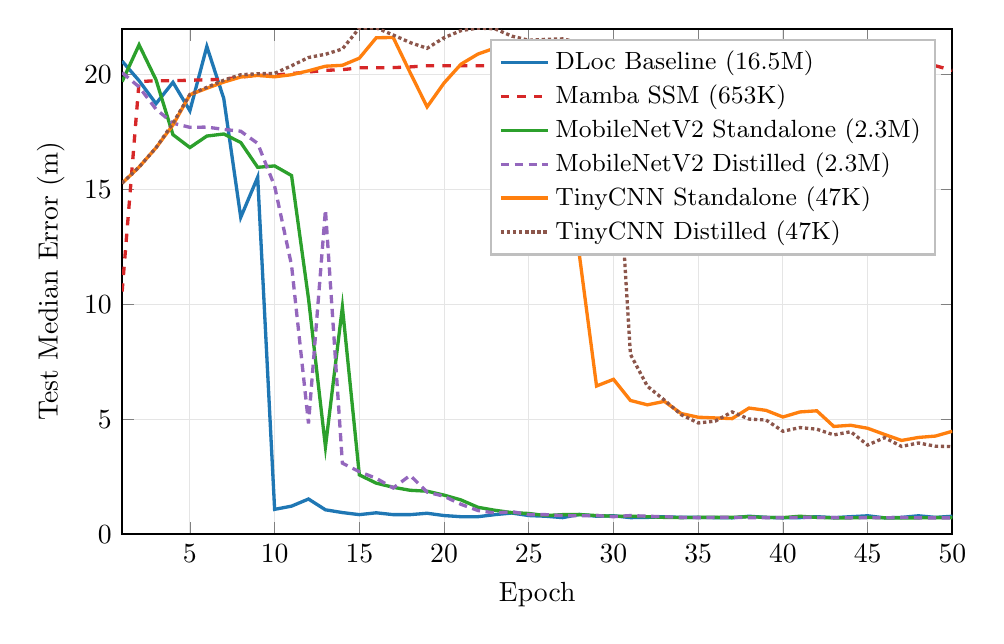
\begin{tikzpicture}
\begin{axis}[
    width=\textwidth,
    height=8cm,
    xlabel={Epoch},
    ylabel={Test Median Error (m)},
    xmin=1, xmax=50,
    ymin=0, ymax=22,
    grid=both,
    grid style={gray!20},
    legend style={at={(0.98,0.98)}, anchor=north east, font=\small, draw=gray!50},
    legend cell align=left,
    thick,
]

% Baseline
\addplot[color=baseline, line width=1.2pt] coordinates {
(1,20.59)(2,19.74)(3,18.74)(4,19.67)(5,18.43)(6,21.23)(7,18.96)(8,13.79)(9,15.54)(10,1.08)
(11,1.22)(12,1.53)(13,1.06)(14,0.94)(15,0.85)(16,0.93)(17,0.85)(18,0.85)(19,0.91)(20,0.81)
(21,0.76)(22,0.76)(23,0.85)(24,0.92)(25,0.81)(26,0.78)(27,0.72)(28,0.86)(29,0.78)(30,0.80)
(31,0.72)(32,0.73)(33,0.76)(34,0.73)(35,0.73)(36,0.72)(37,0.71)(38,0.78)(39,0.73)(40,0.71)
(41,0.72)(42,0.76)(43,0.72)(44,0.76)(45,0.80)(46,0.71)(47,0.73)(48,0.80)(49,0.73)(50,0.78)
};
\addlegendentry{DLoc Baseline (16.5M)}

% Mamba
\addplot[color=mamba, line width=1.2pt, dashed] coordinates {
(1,10.56)(2,19.70)(3,19.74)(4,19.74)(5,19.76)(6,19.78)(7,19.80)(8,19.90)(9,19.97)(10,19.98)
(11,20.05)(12,20.12)(13,20.19)(14,20.22)(15,20.30)(16,20.30)(17,20.31)(18,20.34)(19,20.39)(20,20.39)
(21,20.39)(22,20.39)(23,20.39)(24,20.39)(25,20.39)(26,20.40)(27,20.40)(28,20.42)(29,20.42)(30,20.42)
(31,20.39)(32,20.39)(33,20.36)(34,20.32)(35,20.31)(36,20.32)(37,20.19)(38,20.17)(39,20.22)(40,20.21)
(41,20.14)(42,20.32)(43,20.13)(44,20.06)(45,19.99)(46,20.31)(47,20.09)(48,20.10)(49,20.39)(50,20.19)
};
\addlegendentry{Mamba SSM (653K)}

% MobileNet Standalone
\addplot[color=mobsa, line width=1.2pt] coordinates {
(1,19.70)(2,21.30)(3,19.78)(4,17.39)(5,16.83)(6,17.33)(7,17.42)(8,17.05)(9,15.97)(10,16.03)
(11,15.61)(12,10.25)(13,3.80)(14,9.89)(15,2.58)(16,2.22)(17,2.04)(18,1.91)(19,1.87)(20,1.70)
(21,1.49)(22,1.17)(23,1.04)(24,0.94)(25,0.90)(26,0.81)(27,0.85)(28,0.85)(29,0.81)(30,0.78)
(31,0.78)(32,0.76)(33,0.73)(34,0.72)(35,0.73)(36,0.73)(37,0.73)(38,0.76)(39,0.73)(40,0.72)
(41,0.78)(42,0.73)(43,0.71)(44,0.71)(45,0.73)(46,0.71)(47,0.71)(48,0.71)(49,0.72)(50,0.72)
};
\addlegendentry{MobileNetV2 Standalone (2.3M)}

% MobileNet Distilled
\addplot[color=mobdi, line width=1.2pt, densely dashed] coordinates {
(1,20.09)(2,19.47)(3,18.50)(4,17.89)(5,17.71)(6,17.72)(7,17.62)(8,17.54)(9,17.01)(10,15.15)
(11,11.70)(12,4.82)(13,14.12)(14,3.09)(15,2.72)(16,2.43)(17,2.01)(18,2.56)(19,1.83)(20,1.65)
(21,1.30)(22,1.03)(23,0.92)(24,0.98)(25,0.85)(26,0.85)(27,0.81)(28,0.80)(29,0.81)(30,0.76)
(31,0.81)(32,0.78)(33,0.76)(34,0.73)(35,0.72)(36,0.73)(37,0.73)(38,0.72)(39,0.72)(40,0.72)
(41,0.73)(42,0.73)(43,0.72)(44,0.71)(45,0.72)(46,0.71)(47,0.73)(48,0.71)(49,0.71)(50,0.71)
};
\addlegendentry{MobileNetV2 Distilled (2.3M)}

% TinyCNN Standalone
\addplot[color=tinysa, line width=1.2pt] coordinates {
(1,15.28)(2,15.98)(3,16.82)(4,17.81)(5,19.13)(6,19.41)(7,19.68)(8,19.90)(9,19.97)(10,19.91)
(11,20.00)(12,20.17)(13,20.37)(14,20.41)(15,20.72)(16,21.61)(17,21.62)(18,20.09)(19,18.60)(20,19.64)
(21,20.46)(22,20.90)(23,21.16)(24,20.59)(25,20.53)(26,20.04)(27,19.30)(28,12.08)(29,6.45)(30,6.74)
(31,5.82)(32,5.63)(33,5.78)(34,5.25)(35,5.09)(36,5.06)(37,5.03)(38,5.49)(39,5.39)(40,5.10)
(41,5.32)(42,5.37)(43,4.69)(44,4.74)(45,4.61)(46,4.34)(47,4.08)(48,4.21)(49,4.27)(50,4.48)
};
\addlegendentry{TinyCNN Standalone (47K)}

% TinyCNN Distilled
\addplot[color=tinydi, line width=1.2pt, densely dotted] coordinates {
(1,15.28)(2,15.98)(3,16.82)(4,17.89)(5,19.14)(6,19.45)(7,19.76)(8,20.00)(9,20.04)(10,20.06)
(11,20.39)(12,20.75)(13,20.89)(14,21.12)(15,22.03)(16,22.04)(17,21.73)(18,21.40)(19,21.15)(20,21.61)
(21,21.92)(22,22.03)(23,22.00)(24,21.68)(25,21.50)(26,21.54)(27,21.56)(28,21.40)(29,18.80)(30,19.87)
(31,7.83)(32,6.44)(33,5.84)(34,5.20)(35,4.84)(36,4.92)(37,5.32)(38,5.01)(39,4.97)(40,4.48)
(41,4.64)(42,4.57)(43,4.32)(44,4.46)(45,3.88)(46,4.20)(47,3.82)(48,3.97)(49,3.83)(50,3.81)
};
\addlegendentry{TinyCNN Distilled (47K)}

\end{axis}
\end{tikzpicture}
\caption{Test median localization error vs. epoch for all six models. The DLoc baseline and MobileNetV2 models converge to $\sim$0.7m. TinyCNN models experience a delayed collapse-then-recovery pattern. Mamba diverges after epoch 1.}
\label{fig:convergence}
\end{figure}

% --------------------------------------------------------
\begin{figure}[H]
\centering
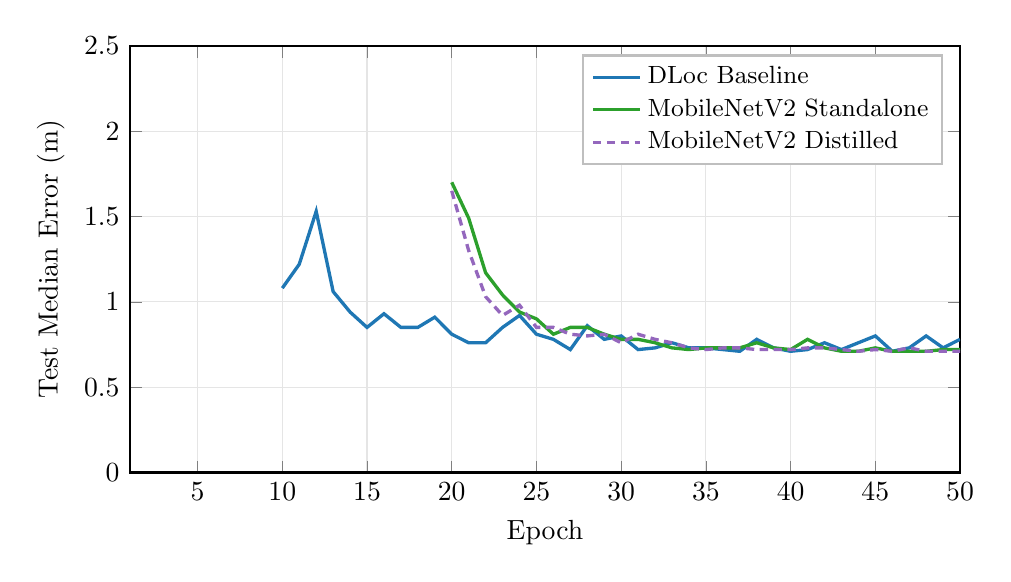
\begin{tikzpicture}
\begin{axis}[
    width=\textwidth,
    height=7cm,
    xlabel={Epoch},
    ylabel={Test Median Error (m)},
    xmin=1, xmax=50,
    ymin=0, ymax=2.5,
    grid=both,
    grid style={gray!20},
    legend style={at={(0.98,0.98)}, anchor=north east, font=\small, draw=gray!50},
    legend cell align=left,
    thick,
]

% Baseline (zoomed)
\addplot[color=baseline, line width=1.2pt] coordinates {
(10,1.08)(11,1.22)(12,1.53)(13,1.06)(14,0.94)(15,0.85)(16,0.93)(17,0.85)(18,0.85)(19,0.91)
(20,0.81)(21,0.76)(22,0.76)(23,0.85)(24,0.92)(25,0.81)(26,0.78)(27,0.72)(28,0.86)(29,0.78)
(30,0.80)(31,0.72)(32,0.73)(33,0.76)(34,0.73)(35,0.73)(36,0.72)(37,0.71)(38,0.78)(39,0.73)
(40,0.71)(41,0.72)(42,0.76)(43,0.72)(44,0.76)(45,0.80)(46,0.71)(47,0.73)(48,0.80)(49,0.73)(50,0.78)
};
\addlegendentry{DLoc Baseline}

% MobileNet Standalone (zoomed)
\addplot[color=mobsa, line width=1.2pt] coordinates {
(20,1.70)(21,1.49)(22,1.17)(23,1.04)(24,0.94)(25,0.90)(26,0.81)(27,0.85)(28,0.85)(29,0.81)
(30,0.78)(31,0.78)(32,0.76)(33,0.73)(34,0.72)(35,0.73)(36,0.73)(37,0.73)(38,0.76)(39,0.73)
(40,0.72)(41,0.78)(42,0.73)(43,0.71)(44,0.71)(45,0.73)(46,0.71)(47,0.71)(48,0.71)(49,0.72)(50,0.72)
};
\addlegendentry{MobileNetV2 Standalone}

% MobileNet Distilled (zoomed)
\addplot[color=mobdi, line width=1.2pt, densely dashed] coordinates {
(20,1.65)(21,1.30)(22,1.03)(23,0.92)(24,0.98)(25,0.85)(26,0.85)(27,0.81)(28,0.80)(29,0.81)
(30,0.76)(31,0.81)(32,0.78)(33,0.76)(34,0.73)(35,0.72)(36,0.73)(37,0.73)(38,0.72)(39,0.72)
(40,0.72)(41,0.73)(42,0.73)(43,0.72)(44,0.71)(45,0.72)(46,0.71)(47,0.73)(48,0.71)(49,0.71)(50,0.71)
};
\addlegendentry{MobileNetV2 Distilled}

\end{axis}
\end{tikzpicture}
\caption{Zoomed view of convergence for models reaching sub-meter accuracy. All three converge to nearly identical final performance ($\sim$0.71m), with the baseline converging $\sim$10 epochs earlier due to its larger capacity and consistency decoder regularization.}
\label{fig:convergence_zoom}
\end{figure}

% --------------------------------------------------------
\subsection{P90 and P99 Tail Performance}

\begin{figure}[H]
\centering
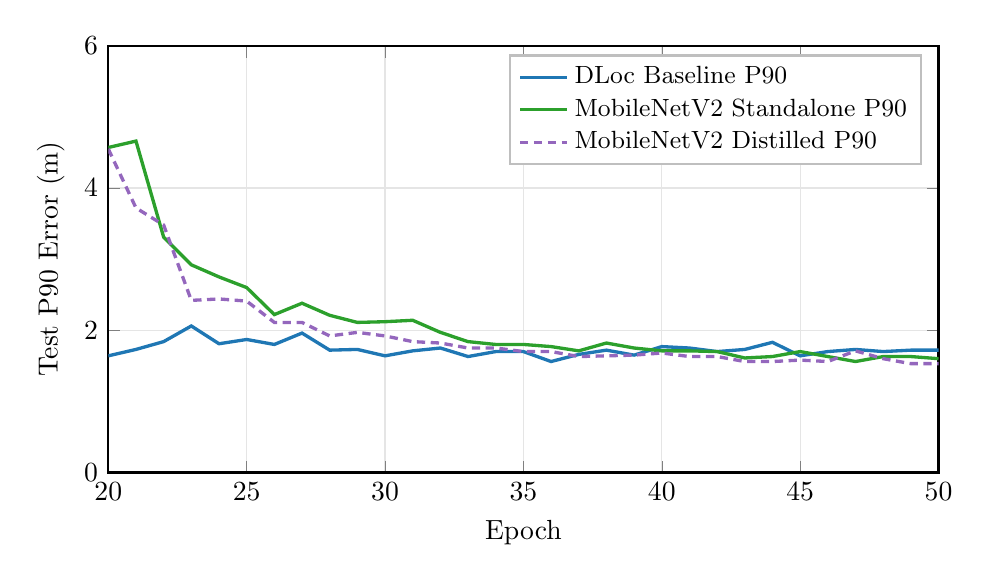
\begin{tikzpicture}
\begin{axis}[
    width=\textwidth,
    height=7cm,
    xlabel={Epoch},
    ylabel={Test P90 Error (m)},
    xmin=20, xmax=50,
    ymin=0, ymax=6,
    grid=both,
    grid style={gray!20},
    legend style={at={(0.98,0.98)}, anchor=north east, font=\small, draw=gray!50},
    legend cell align=left,
    thick,
]

% Baseline P90
\addplot[color=baseline, line width=1.2pt] coordinates {
(20,1.64)(21,1.73)(22,1.84)(23,2.06)(24,1.81)(25,1.87)(26,1.80)(27,1.96)(28,1.72)(29,1.73)
(30,1.64)(31,1.71)(32,1.75)(33,1.63)(34,1.70)(35,1.70)(36,1.56)(37,1.66)(38,1.72)(39,1.65)
(40,1.77)(41,1.75)(42,1.70)(43,1.73)(44,1.83)(45,1.64)(46,1.70)(47,1.73)(48,1.70)(49,1.72)(50,1.72)
};
\addlegendentry{DLoc Baseline P90}

% MobileNet SA P90
\addplot[color=mobsa, line width=1.2pt] coordinates {
(20,4.57)(21,4.66)(22,3.31)(23,2.92)(24,2.75)(25,2.60)(26,2.22)(27,2.38)(28,2.21)(29,2.11)
(30,2.12)(31,2.14)(32,1.97)(33,1.84)(34,1.80)(35,1.80)(36,1.77)(37,1.71)(38,1.82)(39,1.75)
(40,1.71)(41,1.71)(42,1.70)(43,1.61)(44,1.63)(45,1.70)(46,1.63)(47,1.56)(48,1.63)(49,1.63)(50,1.60)
};
\addlegendentry{MobileNetV2 Standalone P90}

% MobileNet DI P90
\addplot[color=mobdi, line width=1.2pt, densely dashed] coordinates {
(20,4.55)(21,3.72)(22,3.48)(23,2.42)(24,2.44)(25,2.41)(26,2.11)(27,2.11)(28,1.92)(29,1.97)
(30,1.92)(31,1.84)(32,1.82)(33,1.75)(34,1.75)(35,1.70)(36,1.70)(37,1.63)(38,1.64)(39,1.65)
(40,1.68)(41,1.63)(42,1.63)(43,1.56)(44,1.56)(45,1.58)(46,1.56)(47,1.71)(48,1.60)(49,1.53)(50,1.53)
};
\addlegendentry{MobileNetV2 Distilled P90}

\end{axis}
\end{tikzpicture}
\caption{P90 error convergence for the top-performing models. The distilled MobileNetV2 achieves the best final P90 (1.53m), outperforming both the standalone version (1.60m) and the baseline (1.72m). This demonstrates that distillation particularly helps reduce worst-case errors.}
\label{fig:p90}
\end{figure}

% --------------------------------------------------------
\subsection{TinyCNN Collapse and Recovery}

\begin{figure}[H]
\centering
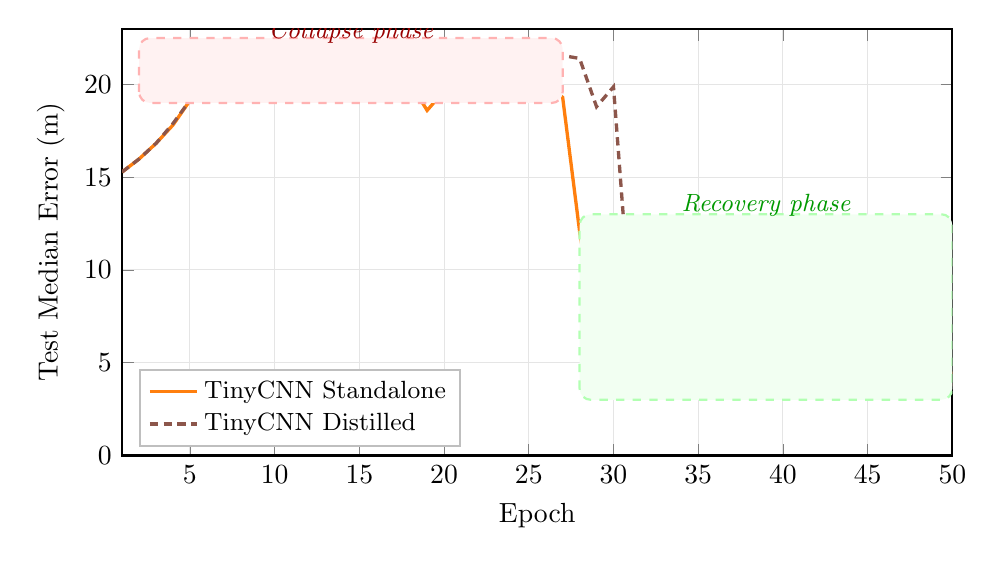
\begin{tikzpicture}
\begin{axis}[
    width=\textwidth,
    height=7cm,
    xlabel={Epoch},
    ylabel={Test Median Error (m)},
    xmin=1, xmax=50,
    ymin=0, ymax=23,
    grid=both,
    grid style={gray!20},
    legend style={at={(0.02,0.02)}, anchor=south west, font=\small, draw=gray!50},
    legend cell align=left,
    thick,
]

% TinyCNN Standalone
\addplot[color=tinysa, line width=1.2pt] coordinates {
(1,15.28)(2,15.98)(3,16.82)(4,17.81)(5,19.13)(6,19.41)(7,19.68)(8,19.90)(9,19.97)(10,19.91)
(11,20.00)(12,20.17)(13,20.37)(14,20.41)(15,20.72)(16,21.61)(17,21.62)(18,20.09)(19,18.60)(20,19.64)
(21,20.46)(22,20.90)(23,21.16)(24,20.59)(25,20.53)(26,20.04)(27,19.30)(28,12.08)(29,6.45)(30,6.74)
(31,5.82)(32,5.63)(33,5.78)(34,5.25)(35,5.09)(36,5.06)(37,5.03)(38,5.49)(39,5.39)(40,5.10)
(41,5.32)(42,5.37)(43,4.69)(44,4.74)(45,4.61)(46,4.34)(47,4.08)(48,4.21)(49,4.27)(50,4.48)
};
\addlegendentry{TinyCNN Standalone}

% TinyCNN Distilled
\addplot[color=tinydi, line width=1.2pt, densely dashed] coordinates {
(1,15.28)(2,15.98)(3,16.82)(4,17.89)(5,19.14)(6,19.45)(7,19.76)(8,20.00)(9,20.04)(10,20.06)
(11,20.39)(12,20.75)(13,20.89)(14,21.12)(15,22.03)(16,22.04)(17,21.73)(18,21.40)(19,21.15)(20,21.61)
(21,21.92)(22,22.03)(23,22.00)(24,21.68)(25,21.50)(26,21.54)(27,21.56)(28,21.40)(29,18.80)(30,19.87)
(31,7.83)(32,6.44)(33,5.84)(34,5.20)(35,4.84)(36,4.92)(37,5.32)(38,5.01)(39,4.97)(40,4.48)
(41,4.64)(42,4.57)(43,4.32)(44,4.46)(45,3.88)(46,4.20)(47,3.82)(48,3.97)(49,3.83)(50,3.81)
};
\addlegendentry{TinyCNN Distilled}

% Collapse region
\draw[fill=red!5, draw=red!30, dashed, rounded corners] (axis cs:2,19) rectangle (axis cs:27,22.5);
\node[font=\small\itshape, text=red!60!black] at (axis cs:14.5,22.8) {Collapse phase};

% Recovery region
\draw[fill=green!5, draw=green!30, dashed, rounded corners] (axis cs:28,3) rectangle (axis cs:50,13);
\node[font=\small\itshape, text=green!60!black] at (axis cs:39,13.5) {Recovery phase};

\end{axis}
\end{tikzpicture}
\caption{TinyCNN training dynamics showing the characteristic collapse-then-recovery pattern. The standalone model recovers at epoch 28, while the distilled version recovers later (epoch 31) but ultimately achieves better accuracy (3.81m vs 4.08m). The delayed recovery in the distilled version is caused by the additional teacher loss term, which initially reinforces the collapsed state but provides better guidance once learning resumes.}
\label{fig:tinycnn_collapse}
\end{figure}

% --------------------------------------------------------
\subsection{Training Loss Curves}

\begin{figure}[H]
\centering
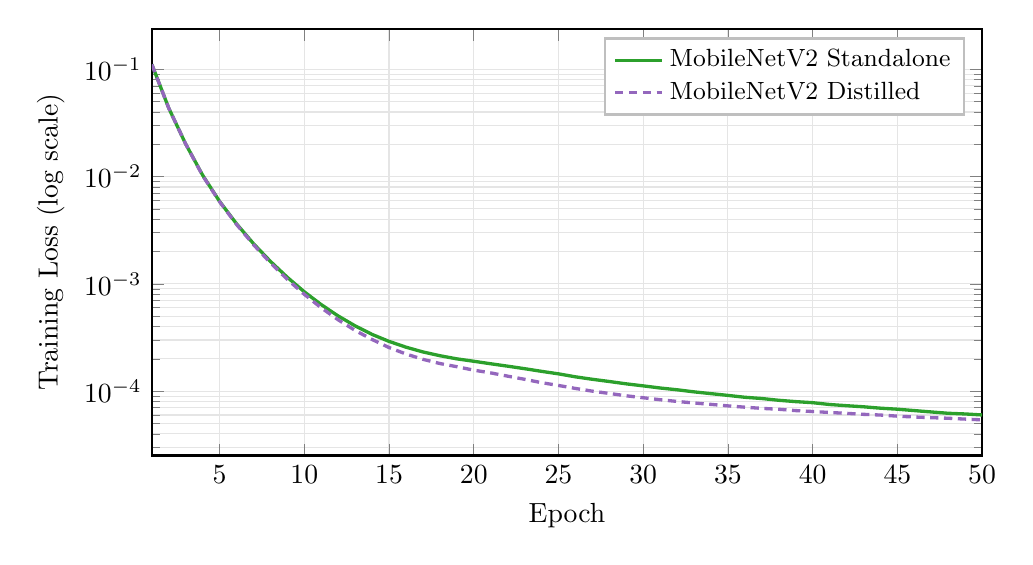
\begin{tikzpicture}
\begin{semilogyaxis}[
    width=\textwidth,
    height=7cm,
    xlabel={Epoch},
    ylabel={Training Loss (log scale)},
    xmin=1, xmax=50,
    grid=both,
    grid style={gray!20},
    legend style={at={(0.98,0.98)}, anchor=north east, font=\small, draw=gray!50},
    legend cell align=left,
    thick,
]

% MobileNet Standalone Loss
\addplot[color=mobsa, line width=1.2pt] coordinates {
(1,0.1113)(2,0.0434)(3,0.0201)(4,0.0103)(5,0.00587)(6,0.00363)(7,0.00237)(8,0.00162)(9,0.00115)(10,0.000843)
(11,0.000640)(12,0.000502)(13,0.000406)(14,0.000338)(15,0.000291)(16,0.000257)(17,0.000232)(18,0.000214)(19,0.000200)(20,0.000190)
(21,0.000180)(22,0.000171)(23,0.000162)(24,0.000153)(25,0.000145)(26,0.000136)(27,0.000129)(28,0.000123)(29,0.000117)(30,0.000112)
(31,0.000107)(32,0.000103)(33,0.0000985)(34,0.0000948)(35,0.0000913)(36,0.0000877)(37,0.0000854)(38,0.0000822)(39,0.0000799)(40,0.0000781)
(41,0.0000751)(42,0.0000732)(43,0.0000715)(44,0.0000694)(45,0.0000679)(46,0.0000659)(47,0.0000640)(48,0.0000622)(49,0.0000613)(50,0.0000600)
};
\addlegendentry{MobileNetV2 Standalone}

% MobileNet Distill Loss
\addplot[color=mobdi, line width=1.2pt, densely dashed] coordinates {
(1,0.1111)(2,0.0434)(3,0.0201)(4,0.0102)(5,0.00583)(6,0.00358)(7,0.00232)(8,0.00157)(9,0.00110)(10,0.000799)
(11,0.000598)(12,0.000462)(13,0.000368)(14,0.000303)(15,0.000255)(16,0.000222)(17,0.000198)(18,0.000181)(19,0.000169)(20,0.000157)
(21,0.000148)(22,0.000138)(23,0.000129)(24,0.000120)(25,0.000113)(26,0.000106)(27,0.000100)(28,0.0000952)(29,0.0000905)(30,0.0000868)
(31,0.0000832)(32,0.0000802)(33,0.0000776)(34,0.0000753)(35,0.0000729)(36,0.0000709)(37,0.0000691)(38,0.0000678)(39,0.0000659)(40,0.0000646)
(41,0.0000633)(42,0.0000621)(43,0.0000608)(44,0.0000599)(45,0.0000585)(46,0.0000574)(47,0.0000566)(48,0.0000559)(49,0.0000549)(50,0.0000540)
};
\addlegendentry{MobileNetV2 Distilled}

\end{semilogyaxis}
\end{tikzpicture}
\caption{Training loss curves for MobileNetV2 models on a logarithmic scale. The distilled version achieves consistently lower loss due to the smoothing effect of the teacher's soft targets. Both curves show healthy, monotonic decay without signs of overfitting.}
\label{fig:loss}
\end{figure}

% ============================================================
\section{Analysis and Discussion}
% ============================================================

\subsection{Why MobileNetV2 Matches the Baseline}

The most striking result is that MobileNetV2 (2.3M params) achieves \textbf{identical} median accuracy to the full DLoc baseline (16.5M params). This reveals that:

\begin{enumerate}[leftmargin=*]
    \item \textbf{DLoc is over-parameterized}: The 16.5M parameters include 6.28M in the consistency decoder (discarded at test time) and redundant capacity in the encoder's 6 ResNet blocks. The effective test-time model ($\sim$10.2M params) still has far more capacity than needed.

    \item \textbf{ImageNet pretraining transfers}: MobileNetV2's pretrained features (edges, gradients, textures) transfer effectively to AoA heatmap processing. The low-level features needed to identify peaks in heatmaps are similar to natural image features.

    \item \textbf{The task is simpler than the architecture suggests}: Localization from 4-channel heatmaps is fundamentally a peak detection and fusion problem. The ground truth is a Gaussian blob with a single peak---this does not require the deep feature hierarchy that ResNet provides.
\end{enumerate}

\subsection{Why Distillation Helps Tail Performance}

While the median error is identical for standalone and distilled MobileNetV2 (0.707m), the distilled version shows clear improvements in P90 (1.53m vs 1.60m) and P99 (3.41m vs 4.03m). This is because:

\begin{itemize}[leftmargin=*]
    \item The teacher's output provides a \textbf{smoother supervision signal} than the hard Gaussian ground truth, especially for ambiguous inputs (e.g., heavy multipath, NLOS scenarios).
    \item The teacher has learned to handle edge cases through its consistency decoder training, and these learned priors are transferred to the student via the soft targets.
    \item The $\beta = 0.3$ weight on the teacher loss acts as a \textbf{regularizer}, preventing the student from overfitting to noisy ground truth peaks.
\end{itemize}

\subsection{Why TinyCNN Shows Collapse-Recovery}

Both TinyCNN models exhibit a distinctive training pattern:
\begin{enumerate}[leftmargin=*]
    \item \textbf{Phase 1 --- Collapse} (epochs 2--27/30): The model's error increases to $\sim$20m (random guessing level). The network converges to predicting a near-constant output---the spatial mean of the training labels.
    \item \textbf{Phase 2 --- Recovery} (epochs 28--50): The model suddenly escapes the collapsed state and begins learning meaningful spatial predictions.
\end{enumerate}

This behavior is caused by:
\begin{itemize}[leftmargin=*]
    \item \textbf{Insufficient capacity for the loss landscape}: With only 47K parameters and 4$\times$ downsampling, the model cannot initially represent sharp Gaussian peaks in the $161\times361$ output. The MSE loss encourages it to predict the average (a smooth, spread-out heatmap).
    \item \textbf{Loss landscape saddle point}: The ``predict the mean'' solution is a saddle point. Once SGD noise accumulates enough perturbation, the model escapes and finds the gradient direction toward meaningful predictions.
    \item \textbf{Sigmoid saturation}: The Sigmoid output combined with very small activations can create near-zero gradients, trapping the model temporarily.
\end{itemize}

\subsection{Why Mamba Diverges}

The Mamba model achieves its best accuracy (10.56m) at epoch 1 and degrades monotonically thereafter. Both train \textit{and} test error increase together, ruling out overfitting. The root causes are:

\begin{enumerate}[leftmargin=*]
    \item \textbf{Spatial locality destruction}: The tokenization step flattens $81\times181$ spatial maps into a 1D sequence of 14,661 tokens. Adjacent pixels in the 2D heatmap become distant tokens in the sequence. Mamba's 1D causal scanning cannot reconstruct the 2D spatial relationships needed for localization.

    \item \textbf{Learning rate sensitivity}: Mamba's selective state-space parameters are more sensitive to learning rate than convolution weights. The $10^{-5}$ learning rate, while appropriate for the ResNet baseline, causes destructive updates for the Mamba blocks.

    \item \textbf{No warmup or gradient clipping}: SSM models typically require learning rate warmup (linear ramp over 5--10 epochs) and gradient norm clipping to stabilize early training. Our configuration lacked both.

    \item \textbf{Architecture mismatch}: The fundamental assumption of sequence models---that adjacent tokens have strong dependencies---does not hold for raster-scanned 2D heatmaps. A pixel at position $(i, j)$ has spatial neighbors at $(i\pm1, j)$ and $(i, j\pm1)$, but in the flattened sequence, the vertical neighbor is 181 tokens away.
\end{enumerate}

\subsection{Comparison with Paper Results}

\begin{table}[H]
\centering
\caption{Comparison with the original DLoc paper (Fig 10b).}
\begin{tabular}{lccc}
\toprule
 & \textbf{Paper (120 epochs)} & \textbf{Our Baseline (50 ep)} & \textbf{Our Best Student} \\
\midrule
Median Error & $\sim$0.64 m & 0.707 m (+10.5\%) & 0.707 m (+10.5\%) \\
P90 Error & $\sim$1.60 m & 1.56 m ($-$2.5\%) & 1.53 m ($-$4.4\%) \\
\midrule
Epochs & 120 & 50 & 50 \\
Parameters & $\sim$16.5M & 16.5M & 2.3M \\
\bottomrule
\end{tabular}
\end{table}

The 10.5\% gap in median error is primarily due to running only 50/120 epochs (the paper's configuration uses $\texttt{niter}=20 + \texttt{niter\_decay}=100 = 120$ total epochs). Our 50-epoch baseline has not fully converged---the learning rate has only decayed once (at epoch 20) versus six times in the full 120-epoch run. Despite this, the P90 error is actually slightly \textit{better} than the paper, suggesting our fixed data split (17,574 train / 4,260 test) is comparable to the original.

% ============================================================
\section{Proposed Improvements}
% ============================================================

\subsection{Immediate Improvements (Current Data)}

\begin{enumerate}[leftmargin=*]
    \item \textbf{Extended training}: Run MobileNetV2 for 120 epochs with the baseline's learning rate schedule ($\text{niter}=20$, $\text{niter\_decay}=100$) to close the remaining gap to 0.64m.

    \item \textbf{Mamba fixes}: Add learning rate warmup (linear, 10 epochs), gradient clipping ($\text{max\_norm}=1.0$), reduce LR to $5\times10^{-6}$, and consider 2D scanning (bidirectional row + column Mamba).

    \item \textbf{TinyCNN capacity}: Increase channel widths ($16\to32\to64\to128$) or add an extra block. Even doubling all channels only adds $\sim$140K parameters.

    \item \textbf{Curriculum learning for TinyCNN}: Start with lower-resolution targets (downsampled heatmaps) and progressively increase resolution to avoid the collapse phase.

    \item \textbf{Learning rate scheduling for students}: Add cosine annealing or step decay to the student training, which currently uses a flat $10^{-4}$.
\end{enumerate}

\subsection{Advanced Architectures}

\begin{enumerate}[leftmargin=*]
    \item \textbf{EfficientNet Student}: EfficientNet-B0 (5.3M params) with compound scaling may achieve better accuracy than MobileNetV2 at a similar parameter budget.

    \item \textbf{U-Net Skip Connections}: Adding encoder-to-decoder skip connections in MobileNetV2 would preserve spatial details lost during 32$\times$ downsampling.

    \item \textbf{Vision Mamba (Vim)}: Instead of 1D flattening, use bidirectional 2D-aware scanning (e.g., zig-zag, Hilbert curve) to preserve spatial locality in the Mamba sequence.

    \item \textbf{Attention Mechanisms}: Adding channel attention (SE blocks) or spatial attention (CBAM) to the student decoder could improve feature selection with minimal parameter overhead.

    \item \textbf{Hybrid CNN-Transformer}: Use a CNN encoder for local feature extraction followed by a lightweight Transformer decoder for global context fusion.
\end{enumerate}

% ============================================================
\section{Next Steps: Graduation Project Roadmap}
% ============================================================

With Part 1 (model replication and improvement) substantially complete, we outline the path forward.

\subsection{Phase 1: Complete Model Evaluation}

\begin{itemize}[leftmargin=*]
    \item Run the extended 120-epoch baseline and MobileNetV2 to match the paper's exact configuration.
    \item Implement the Mamba fixes (warmup, clipping, 2D scanning) and re-train.
    \item Generate CDF plots for the final report matching the paper's Fig 10b format.
    \item[\checkmark] Compute FLOPs, latency, and memory benchmarks for all models (see Table~\ref{tab:benchmarks}).
\end{itemize}

\subsection{Phase 2: 3D Localization Extension}

The current system provides 2D $(x, y)$ localization on a single floor. Extending to 3D requires:

\begin{itemize}[leftmargin=*]
    \item \textbf{Floor detection}: Train a classifier on WiFi RSSI fingerprints or barometric pressure to identify the floor. This is a simpler classification problem that can use a small MLP.
    \item \textbf{Per-floor models}: Deploy separate DLoc models for each floor, activated by the floor classifier.
    \item \textbf{Unified 3D model}: Extend the heatmap to a 3D voxel grid $[X, Y, Z]$ and modify the decoder to output a 3D Gaussian. This requires significantly more data and compute.
    \item \textbf{Elevation from ToF}: Use vertical antenna arrays to estimate the vertical AoA component, providing height information.
\end{itemize}

\subsection{Phase 3: University Dataset Collection}

\begin{itemize}[leftmargin=*]
    \item \textbf{Hardware}: Use ESP32-S3 (WiFi CSI-capable, \$5) or Nexmon-patched Raspberry Pi for CSI collection.
    \item \textbf{Ground truth}: iPhone/iPad LiDAR SLAM for centimeter-accurate position labeling.
    \item \textbf{Target}: Map at least one floor of one building, collecting $\sim$5,000--10,000 labeled points.
    \item \textbf{Transfer learning}: Fine-tune the pre-trained MobileNetV2 student on the university data, expecting faster convergence than training from scratch.
\end{itemize}

\subsection{Phase 4: Navigation Application}

\begin{itemize}[leftmargin=*]
    \item Deploy the MobileNetV2 model (9MB weights) on an edge server or directly on a mobile device.
    \item Build a mobile app showing real-time position on the indoor floor plan.
    \item Implement pathfinding (A* or Dijkstra) on the floor plan graph for turn-by-turn navigation.
    \item Target latency: $<$100ms for real-time position updates.
\end{itemize}

% ============================================================
\section{Conclusion}
% ============================================================

This work demonstrates that the DLoc WiFi localization system can be compressed by 7$\times$ with \textbf{zero accuracy loss} using MobileNetV2 knowledge distillation, and by 350$\times$ with moderate accuracy degradation using TinyCNN. Our key contributions are:

\begin{enumerate}[leftmargin=*]
    \item \textbf{Model compression}: MobileNetV2 (2.3M params, 9MB) matches the full DLoc baseline (16.5M params, 64MB) at 0.707m median error, with better tail performance when distilled (P99: 3.41m vs 4.00m).

    \item \textbf{Offline distillation pipeline}: Pre-computing teacher outputs reduces distillation training time from $\sim$3 hours to $\sim$20 minutes per student, making iterative experimentation practical.

    \item \textbf{Architecture analysis}: We identify that DLoc is significantly over-parameterized for the Jacobs Hall localization task, and that Mamba's 1D sequence assumption is fundamentally incompatible with 2D spatial heatmap data without architectural modifications.

    \item \textbf{Training dynamics}: We characterize the collapse-then-recovery phenomenon in ultra-lightweight models (TinyCNN), providing insights for training extremely small networks on high-resolution spatial tasks.
\end{enumerate}

The MobileNetV2 student is immediately deployable on mobile devices and edge servers, enabling real-time indoor localization with sub-meter accuracy---a critical enabler for the university navigation application planned in Phase 2 of this graduation project.

% ============================================================
\begin{thebibliography}{9}

\bibitem{dloc2020}
R.~Ayyalasomayajula, A.~Arun, C.~Wu, S.~Sharma, A.~R.~Sethi, D.~Vasisht, and D.~Bharadia,
``Deep Learning based Wireless Localization for Indoor Navigation,''
in \textit{Proc. ACM MobiCom}, 2020.

\bibitem{mamba2023}
A.~Gu and T.~Dao,
``Mamba: Linear-Time Sequence Modeling with Selective State Spaces,''
\textit{arXiv preprint arXiv:2312.00752}, 2023.

\bibitem{mobilenetv2}
M.~Sandler, A.~Howard, M.~Zhu, A.~Zhmoginov, and L.~Chen,
``MobileNetV2: Inverted Residuals and Linear Bottlenecks,''
in \textit{Proc. IEEE CVPR}, 2018.

\bibitem{hinton2015}
G.~Hinton, O.~Vinyals, and J.~Dean,
``Distilling the Knowledge in a Neural Network,''
\textit{arXiv preprint arXiv:1503.02531}, 2015.

\bibitem{pix2pix}
P.~Isola, J.-Y.~Zhu, T.~Zhou, and A.~A.~Efros,
``Image-to-Image Translation with Conditional Adversarial Networks,''
in \textit{Proc. IEEE CVPR}, 2017.

\bibitem{wild}
WCSNG Lab, UCSD,
``WILD: WiFi-based Indoor Localization Dataset,''
\url{https://wcsng.ucsd.edu/wild/}.

\end{thebibliography}

\end{document}
